% !TEX program = xelatex
% 教案例子·进阶：条件 DDPM（MNIST 数字类别作为条件）
\documentclass[a4paper,fontset=none,zihao=5]{ctexart}

\setCJKmainfont{NotoSerifCJK-Regular.ttc}[Path=/usr/share/fonts/opentype/noto/,FontIndex=2,BoldFont=NotoSerifCJK-Bold.ttc,BoldFeatures={FontIndex=2},ItalicFont=NotoSerifCJK-Regular.ttc,ItalicFeatures={FontIndex=2}]
\setCJKsansfont{NotoSansCJK-Regular.ttc}[Path=/usr/share/fonts/opentype/noto/,FontIndex=2,BoldFont=NotoSansCJK-Bold.ttc,BoldFeatures={FontIndex=2}]
\setCJKmonofont{NotoSansCJK-Regular.ttc}[Path=/usr/share/fonts/opentype/noto/,FontIndex=2]
\setmonofont{DejaVu Sans Mono}[Scale=0.93]

\usepackage[margin=1.8cm,top=2.0cm,bottom=2.0cm]{geometry}
\usepackage{amsmath,amssymb,mathtools,bm}
\usepackage{graphicx,float,caption,booktabs,enumitem,array,tabularx}
\usepackage{xcolor}
\usepackage[most]{tcolorbox}
\usepackage{listings}
\usepackage{fancyhdr}
\usepackage[unicode]{hyperref}
\usepackage{xurl}

\definecolor{ctitle}{HTML}{1E3A8A}
\definecolor{chead}{HTML}{1E40AF}
\definecolor{csub}{HTML}{334155}
\definecolor{cbox}{HTML}{EFF6FF}
\definecolor{cboxb}{HTML}{93C5FD}
\definecolor{cnote}{HTML}{9A3412}
\definecolor{cnotebg}{HTML}{FFF7ED}
\definecolor{cmuted}{HTML}{64748B}
\definecolor{cwhy}{HTML}{047857}
\definecolor{cwhybg}{HTML}{ECFDF5}
\definecolor{clink}{HTML}{1D4ED8}
\definecolor{ccodebg}{HTML}{F8FAFC}
\definecolor{ccomment}{HTML}{15803D}
\definecolor{ckw}{HTML}{7C3AED}
\definecolor{cstr}{HTML}{B45309}

\hypersetup{colorlinks=true,linkcolor=chead,urlcolor=clink,citecolor=chead,
  pdftitle={教案例子·进阶：条件 DDPM（MNIST 数字类别作为条件）},
  pdfauthor={Grok Bot 教学笔记}}

\ctexset{
  section = {format=\Large\sffamily\bfseries\color{chead}, name={,}, number=\chinese{section}、, aftername={}, beforeskip=1.1em, afterskip=0.6em},
  subsection = {format=\large\sffamily\bfseries\color{csub}, beforeskip=0.8em, afterskip=0.4em},
}
\pagestyle{fancy}\fancyhf{}
\renewcommand{\headrulewidth}{0.4pt}
\renewcommand{\headrule}{\color{black!15}\hrule height\headrulewidth}
\fancyfoot[C]{\footnotesize\color{cmuted}条件 MNIST DDPM · 进阶教案例子\quad·\quad 第 \thepage{} 页}
\fancypagestyle{plain}{\fancyhf{}\renewcommand{\headrulewidth}{0pt}%
  \fancyfoot[C]{\footnotesize\color{cmuted}条件 MNIST DDPM · 进阶教案例子\quad·\quad 第 \thepage{} 页}}
\captionsetup{font={small,color=cmuted},labelsep=quad}
\captionsetup[figure]{name=图}
\captionsetup[table]{name=表}

\newtcolorbox{notebox}[1][]{enhanced,breakable,colback=cnotebg,colframe=cnote!45,boxrule=0.5pt,arc=2pt,
  left=6pt,right=6pt,top=4pt,bottom=4pt,fontupper=\small\color{cnote},#1}
\newtcolorbox{keybox}[1][]{enhanced,colback=cbox,colframe=cboxb,boxrule=0.6pt,arc=2pt,left=6pt,right=6pt,top=2pt,bottom=2pt,#1}
\newtcolorbox{warnbox}[1][]{enhanced,breakable,colback=red!3,colframe=red!55!black,boxrule=0.6pt,arc=2pt,left=6pt,right=6pt,top=3pt,bottom=3pt,#1}
\newtcolorbox{whybox}[1][]{enhanced,breakable,colback=cwhybg,colframe=cwhy!55,boxrule=0.5pt,arc=2pt,
  left=6pt,right=6pt,top=3pt,bottom=4pt,fontupper=\small,
  title={\sffamily\bfseries 为什么这样做？},coltitle=cwhy,colbacktitle=cwhybg,attach title to upper={\quad},#1}
\newtcolorbox{stepbox}[2][]{enhanced,breakable,colback=white,colframe=chead!60,boxrule=0.6pt,arc=2pt,
  left=6pt,right=6pt,top=3pt,bottom=4pt,title={\sffamily\bfseries #2},colbacktitle=chead!8,coltitle=chead,#1}

\lstdefinestyle{py}{language=Python,basicstyle=\ttfamily\footnotesize,
  backgroundcolor=\color{ccodebg},frame=single,rulecolor=\color{black!15},
  numbers=left,numberstyle=\tiny\color{cmuted},numbersep=6pt,xleftmargin=1.6em,framexleftmargin=1.4em,
  keywordstyle=\color{ckw}\bfseries,commentstyle=\color{ccomment},stringstyle=\color{cstr},
  showstringspaces=false,breaklines=true,columns=fullflexible,keepspaces=true,tabsize=4,upquote=true}
\lstdefinestyle{sh}{basicstyle=\ttfamily\footnotesize,backgroundcolor=\color{ccodebg},frame=single,
  rulecolor=\color{black!15},columns=fullflexible,keepspaces=true,breaklines=true,showstringspaces=false}

\newcommand{\x}{\mathbf{x}}
\newcommand{\I}{\mathbf{I}}
\newcommand{\N}{\mathcal{N}}
\newcommand{\abar}{\bar{\alpha}}
\newcommand{\eps}{\boldsymbol{\epsilon}}
\newcommand{\epst}{\boldsymbol{\epsilon}_\theta}
\newcommand{\E}{\mathbb{E}}
\newcommand{\code}[1]{\texttt{#1}}
\newcommand{\mathnotes}{《扩散生成模型的数学原理》}
\newcommand{\moonslab}{《2D DDPM 动手实验》教案}

\setlength{\parskip}{0.3em}
\setlength{\emergencystretch}{3em}
\linespread{1.22}

\usepackage{rotating}
\begin{document}
\thispagestyle{plain}
\begin{center}
  \vspace*{0.5cm}
  {\sffamily\bfseries\fontsize{20}{28}\selectfont\color{ctitle} 教案例子·进阶：条件扩散模型\par}
  \vspace{0.35em}
  {\large\color{csub} MNIST 手写数字\enspace·\enspace 类别编码为条件\enspace·\enspace Classifier-Free Guidance\par}
  \vspace{0.35em}
  {\color{chead}\rule{0.65\textwidth}{1.5pt}\par}
  \vspace{0.15em}
  {\small\color{cmuted} 前置：\moonslab\quad|\quad 配套数学：\mathnotes\par}
\end{center}

\begin{keybox}
\small
\renewcommand{\arraystretch}{1.25}
\begin{tabularx}{\linewidth}{@{}>{\bfseries}p{0.15\linewidth}X@{}}
课题 & 条件 DDPM：把数字类别 $c\in\{0,\dots,9\}$ 编码进 $\epst(\x_t,t,c)$，按需生成指定数字 \\
对象 & 已完成双月无条件实验的本科高年级 / 研究生 \\
先修 & 双月教案（前向闭式、$\eps$-loss、祖先采样）；PyTorch 卷积基础；讲义第二、四章 \\
时长 & 90–120 分钟（概念 20 + 代码对照 25 + 训练等待/讲解 30 + 采样与 CFG 讨论 20） \\
硬件 & 课堂 GPU：A100 / H200（单卡即可）。\code{classroom\_cond\_mnist.py} 10 epochs \emph{估计} 2–5 分钟（未在 GPU 上实测，脚本会打印真实耗时）；参考：8 核 CPU 实测 8 epochs 27.5 分钟。无时间时直接加载 \code{runs/final/ckpt\_ema.pt} \\
产出 & 0–9 条件采样网格图、CFG 对比图、loss 曲线；能口述「条件如何进入网络」 \\
\end{tabularx}
\end{keybox}

\section{与双月实验的关系}
\begin{center}\small
\renewcommand{\arraystretch}{1.25}
\begin{tabularx}{\linewidth}{@{}lll@{}}
\toprule
 & 双月实验（入门） & 本实验（进阶） \\
\midrule
数据 & 2D 点云 \code{make\_moons} & $28\times28$ 灰度图 MNIST \\
网络 & 小 MLP & U-Net + 7$\times$7 自注意力（约 214 万参数）+ EMA \\
条件 & 无（只学 $p(\x)$） & 有：类别 $c$（学 $p(\x\mid c)$） \\
采样控制 & 只能「随机生成一个双月」 & 可指定「生成数字 3」 \\
新概念 & --- & 类别嵌入、CFG（可选） \\
\bottomrule
\end{tabularx}
\end{center}
数学骨架不变：前向闭式、$\|\eps-\epst\|^2$、反向均值公式。变的是网络输入多了 $c$，以及采样时可选用 guidance。

\section{教学目标}
\begin{enumerate}[leftmargin=2em,itemsep=1pt]
  \item 说清「条件」的含义：网络从 $\epst(\x_t,t)$ 变成 $\epst(\x_t,t,c)$，学的是条件分布 $p(\x_0\mid c)$；
  \item 指出类别嵌入在代码中的位置，并解释为何把它与时间嵌入相加后注入 ResBlock；
  \item 完成带标签的训练循环（含随机丢弃标签以支持 CFG），并按指定数字采样；
  \item （可选）解释 Classifier-Free Guidance：$\hat\eps=\eps_\emptyset+w(\eps_c-\eps_\emptyset)$，并观察 $w$ 对样本的影响。
\end{enumerate}

\section{数学要点（条件版）}
\subsection{条件前向与训练}
前向过程\emph{不依赖}条件（噪声日程与数据标签无关）：
\begin{equation}
  \x_t=\sqrt{\abar_t}\,\x_0+\sqrt{1-\abar_t}\,\eps,\qquad \eps\sim\N(\mathbf 0,\I).
\end{equation}
训练时，每个样本带着它的标签 $c$（MNIST 的 $0$–$9$），网络预测噪声：
\begin{keybox}
\begin{equation}
  L(\theta)=\E_{t,\x_0,c,\eps}\Big[\big\|\eps-\epst(\x_t,t,c)\big\|^2\Big].
  \label{eq:cond-loss}
\end{equation}
\end{keybox}
采样时喂入想要的 $c$，反向均值公式与无条件相同，只是 $\epst$ 多了参数 $c$：
\begin{equation}
  \boldsymbol\mu_\theta(\x_t,t,c)=\frac{1}{\sqrt{\alpha_t}}\Big(\x_t-\frac{\beta_t}{\sqrt{1-\abar_t}}\,\epst(\x_t,t,c)\Big).
\end{equation}

\begin{whybox}
\textbf{为什么前向不加条件、反向才加？}加噪是「破坏信息」的固定物理过程，与「想生成哪个数字」无关；
条件只告诉反向过程「往哪个数据流形去」。这对应贝叶斯视角：真正用到的是 $q(\x_{t-1}\mid\x_t,\x_0)$ 的近似，而 $\x_0$ 的分布换成了条件分布 $q(\x_0\mid c)$——训练时用带标签的样本估计它。
\end{whybox}

\subsection{条件如何进入网络}
本实验用\textbf{类别嵌入}：\code{nn.Embedding(11, emb\_dim)}（下标 $0$–$9$ 为数字，下标 $10$ 为「无条件」空标签）。
\begin{equation}
  \mathbf e(t,c)=\mathrm{MLP}(\mathrm{SinTime}(t))+\mathrm{Embed}(c)\in\mathbb R^{d},
\end{equation}
再把 $\mathbf e$ 加到每个 ResBlock 的特征图上（广播到空间维）。这样「现在是第几步」与「要生成哪个数字」共用同一条条件通道。

\subsection{引导（Guidance）：从 CG 到 CFG}

\subsubsection{为什么还要「引导」？——纯条件模型的不足}
有了 $\epst(\x_t,t,c)$，直接用它做祖先采样（$w=1$）在理论上就是从 $p_\theta(\x_0\mid c)$ 采样。但实践中常见两类现象：
\begin{enumerate}[leftmargin=2em,itemsep=1pt]
  \item \textbf{条件偏弱：}网络容量与训练步数有限时，$p_\theta(\x\mid c)$ 往往比真实的 $p(\x\mid c)$ 更「宽」，会混入其他类的特征——本实验 $w=1$ 时第 5 行偶尔画成 6 状、第 2 行偶尔出现 1/8 状（图~\ref{fig:cfg}）；
  \item \textbf{多样但类别身份模糊：}样本分布覆盖面广（多样性高），但其中一部分「既像 3 又像 8」，按类别看不够典型。
\end{enumerate}
我们想要一个旋钮：牺牲一点多样性，换取更高的\textbf{类别保真度}（fidelity）——即让样本 $\x$ 的后验 $p(c\mid\x)$ 更尖锐、更确信是 $c$。这就是 guidance 的目标：
\begin{equation}
  \tilde p_w(\x\mid c)\ \propto\ p(\x\mid c)\,p(c\mid\x)^{\,w-1}
  \ \propto\ p(\x)\,p(c\mid\x)^{\,w}.
  \label{eq:sharpen}
\end{equation}
$w=1$ 时就是原条件分布；$w>1$ 时，「分类器越确信是 $c$ 的区域」被放大。

\begin{whybox}
\textbf{温度类比。}语言模型里把 softmax 温度调低，会让高概率词更突出、输出更「确定」但更单调；式~\eqref{eq:sharpen} 对 $p(c\mid\x)$ 做的是同一件事（$p^{w}$ 相当于温度 $1/w$）。GAN 里的截断技巧（truncation trick）同样是「多样性换质量」。所以 guidance 不是让模型「更正确」，而是在\emph{保真度—多样性}曲线上选一个点；FID 通常在中等 $w$ 处最好，IS / 分类准确率随 $w$ 单调升高。
\end{whybox}

\subsubsection{Classifier Guidance（CG）：用外部分类器的梯度}
Dhariwal \& Nichol（2021，\href{https://arxiv.org/abs/2105.05233}{arXiv:2105.05233}）的思路是对式~\eqref{eq:sharpen} 取对数再对 $\x_t$ 求梯度（score）。由贝叶斯公式 $p(\x_t\mid c)=p(c\mid\x_t)p(\x_t)/p(c)$，且 $p(c)$ 与 $\x_t$ 无关：
\begin{equation}
  \nabla_{\x_t}\log p(\x_t\mid c)=\nabla_{\x_t}\log p(\x_t)+\nabla_{\x_t}\log p(c\mid\x_t).
  \label{eq:bayes-score}
\end{equation}
扩散模型的噪声预测与 score 的关系是 $\nabla_{\x_t}\log p_t(\x_t)\approx-\epst(\x_t,t)/\sqrt{1-\abar_t}$（讲义 score 一节）。把分类器项乘上引导强度 $s$ 后换回 $\eps$ 记号：
\begin{keybox}
\begin{equation}
  \tilde\eps(\x_t,t,c)=\epst(\x_t,t)-\sqrt{1-\abar_t}\;s\;\nabla_{\x_t}\log p_\phi(c\mid\x_t).
  \label{eq:cg}
\end{equation}
\end{keybox}
它对应的目标分布是 $p(\x_t)\,p_\phi(c\mid\x_t)^{s}$，即式~\eqref{eq:sharpen} 中 $w=s$。若底座本身已是条件模型 $\epst(\x_t,t,c)$，则对应 $p(\x_t\mid c)\,p_\phi(c\mid\x_t)^{s}$，相当于 $w=1+s$。

\textbf{CG 的代价：}
\begin{itemize}[leftmargin=1.6em,itemsep=1pt]
  \item \textbf{要额外训练一个「噪声感知」分类器} $p_\phi(c\mid\x_t,t)$：普通 MNIST 分类器只见过干净图，在 $t$ 很大的 $\x_t$ 上输出没有意义，必须在加噪数据上（输入含 $t$）重新训练；
  \item \textbf{每步要对分类器反向传播}求输入梯度，采样成本与显存都增加；
  \item \textbf{梯度可能「对抗」：}分类器的输入梯度容易指向人眼不可见的微小扰动（类似对抗样本），能提高分类器分数却不一定改善图像；
  \item 引导质量受限于分类器本身，换一种条件（如文本）就要再训一个对应的「分类器」。
\end{itemize}

\subsubsection{从 CG 推出 CFG：把分类器「藏」进生成模型}
Ho \& Salimans（2022，\href{https://arxiv.org/abs/2207.12598}{arXiv:2207.12598}）注意到，式~\eqref{eq:bayes-score} 可以反过来用：\emph{隐式分类器}的梯度等于两个生成模型 score 之差，
\begin{equation}
  \nabla_{\x_t}\log p(c\mid\x_t)=\nabla_{\x_t}\log p(\x_t\mid c)-\nabla_{\x_t}\log p(\x_t)
  \approx-\frac{1}{\sqrt{1-\abar_t}}\Big(\epst(\x_t,t,c)-\epst(\x_t,t,\emptyset)\Big).
\end{equation}
代入式~\eqref{eq:cg}（底座取无条件 $\eps_\emptyset$，强度记作 $w$），$\sqrt{1-\abar_t}$ 恰好约掉：
\begin{keybox}
\begin{equation}
  \hat\eps=\eps_\theta(\x_t,t,\emptyset)+w\big(\eps_\theta(\x_t,t,c)-\eps_\theta(\x_t,t,\emptyset)\big).
  \label{eq:cfg}
\end{equation}
\end{keybox}
\textbf{$w$ 与 $s$ 的对应：}以无条件模型为底座时 $w=s$；Ho \& Salimans 原文写成 $(1+w')\eps_c-w'\eps_\emptyset$，即 $w=1+w'$。本教案统一用式~\eqref{eq:cfg} 的 $w$：$w=1$ 为纯条件。

\textbf{一个网络同时学 $\eps_c$ 与 $\eps_\emptyset$：}训练时以概率 $p_{\mathrm{uncond}}=0.1$ 把标签换成空标签 $\emptyset$（代码中下标 $10$，\code{nn.Embedding(11,128)} 的第 11 行）。于是同一组参数在 90\% 的样本上学条件 score、10\% 上学无条件 score，采样时只需换输入标签就能得到两者。

\begin{whybox}
\textbf{为什么丢弃率取 0.1 左右？}太小（如 0.01）则无条件分支训练样本太少，$\eps_\emptyset$ 不准，差值 $\eps_c-\eps_\emptyset$ 噪声大；太大（如 0.5）则条件分支少了一半数据，$w=1$ 的质量下降。原文在 0.1–0.2 之间效果相近，0.1 是常用折中。\\
\textbf{为什么叫「无分类器」？}引导方向 $\eps_c-\eps_\emptyset$ 由生成模型自己给出，不需要外部分类器、不需要对输入求梯度——只是多一次前向，且没有对抗梯度问题。
\end{whybox}

\subsubsection{$w$ 的作用与本实验的实测}
\begin{itemize}[leftmargin=1.6em,itemsep=1pt]
  \item $w=0$：$\hat\eps=\eps_\emptyset$，完全忽略 $c$，即无条件生成（随机数字）；
  \item $w=1$：纯条件模型，$\hat\eps=\eps_c$；
  \item $w>1$：沿「条件减无条件」方向外推，对应式~\eqref{eq:sharpen} 的锐化。
\end{itemize}
本实验同一模型、同一随机种子下（\code{runs/final/samples\_g1.png}、\code{samples\_g1.5.png}、\code{samples\_g3.png}，图~\ref{fig:cfg}），用小 CNN 分类器（测试集 98.83\%）判卷、每类 30 张：$w=1$ 总体 \textbf{95.0\%}（最弱为数字 5：26/30），$w=1.5$ 为 \textbf{100\%}（300/300），见表~\ref{tab:clf}。肉眼看 $w=3$ 的网格笔画更粗、同一行更「整齐划一」，多样性明显下降。
\begin{whybox}
\textbf{大 $w$ 的副作用与 $\hat\x_0$ 裁剪。}外推使 $\hat\eps$ 的幅度超出训练时见过的范围，由它算出的 $\hat\x_0=(\x_t-\sqrt{1-\abar_t}\hat\eps)/\sqrt{\abar_t}$ 容易跑出 $[-1,1]$，表现为过饱和、笔画发胖。本实验采样时先把 $\hat\x_0$ 裁剪到 $[-1,1]$ 再算后验均值，这能防止像素「爆掉」，但也会把过度外推「压平」——所以大 $w$ 下看到的是粗而整齐的数字，而不是噪点。修复前的小模型在 $w=3$ 且未裁剪时出现过整行全黑，就是这种外推失控的极端情况。
\end{whybox}


\subsubsection{对照：没有类别条件时（$w=0$ / null 标签）}
若采样时始终喂空标签 $\emptyset$（代码中 $c=10$），则 $\hat\eps=\eps_\emptyset$，完全忽略想要的数字——这就是式~\eqref{eq:cfg} 里 $w=0$ 的情形。用同一份 EMA 权重（\code{runs/final/ckpt\_ema.pt}）实测采样 100 张（10$\times$10 网格，耗时 144.7 s）：
\begin{itemize}[leftmargin=1.6em,itemsep=0pt]
  \item 样本仍然是清晰的手写数字（模型学到了 $p(\x)$）；
  \item 但各类别\emph{混在每一行}——行标签只是排版，不是条件（图~\ref{fig:uncond}）；
  \item 对比同权重下 $w=1$（纯条件，分类器 95.0\%）与 $w=1.5$（CFG，100\%）：没有条件就无法「指定生成数字 3」。
\end{itemize}
\begin{figure}[H]
  \centering
  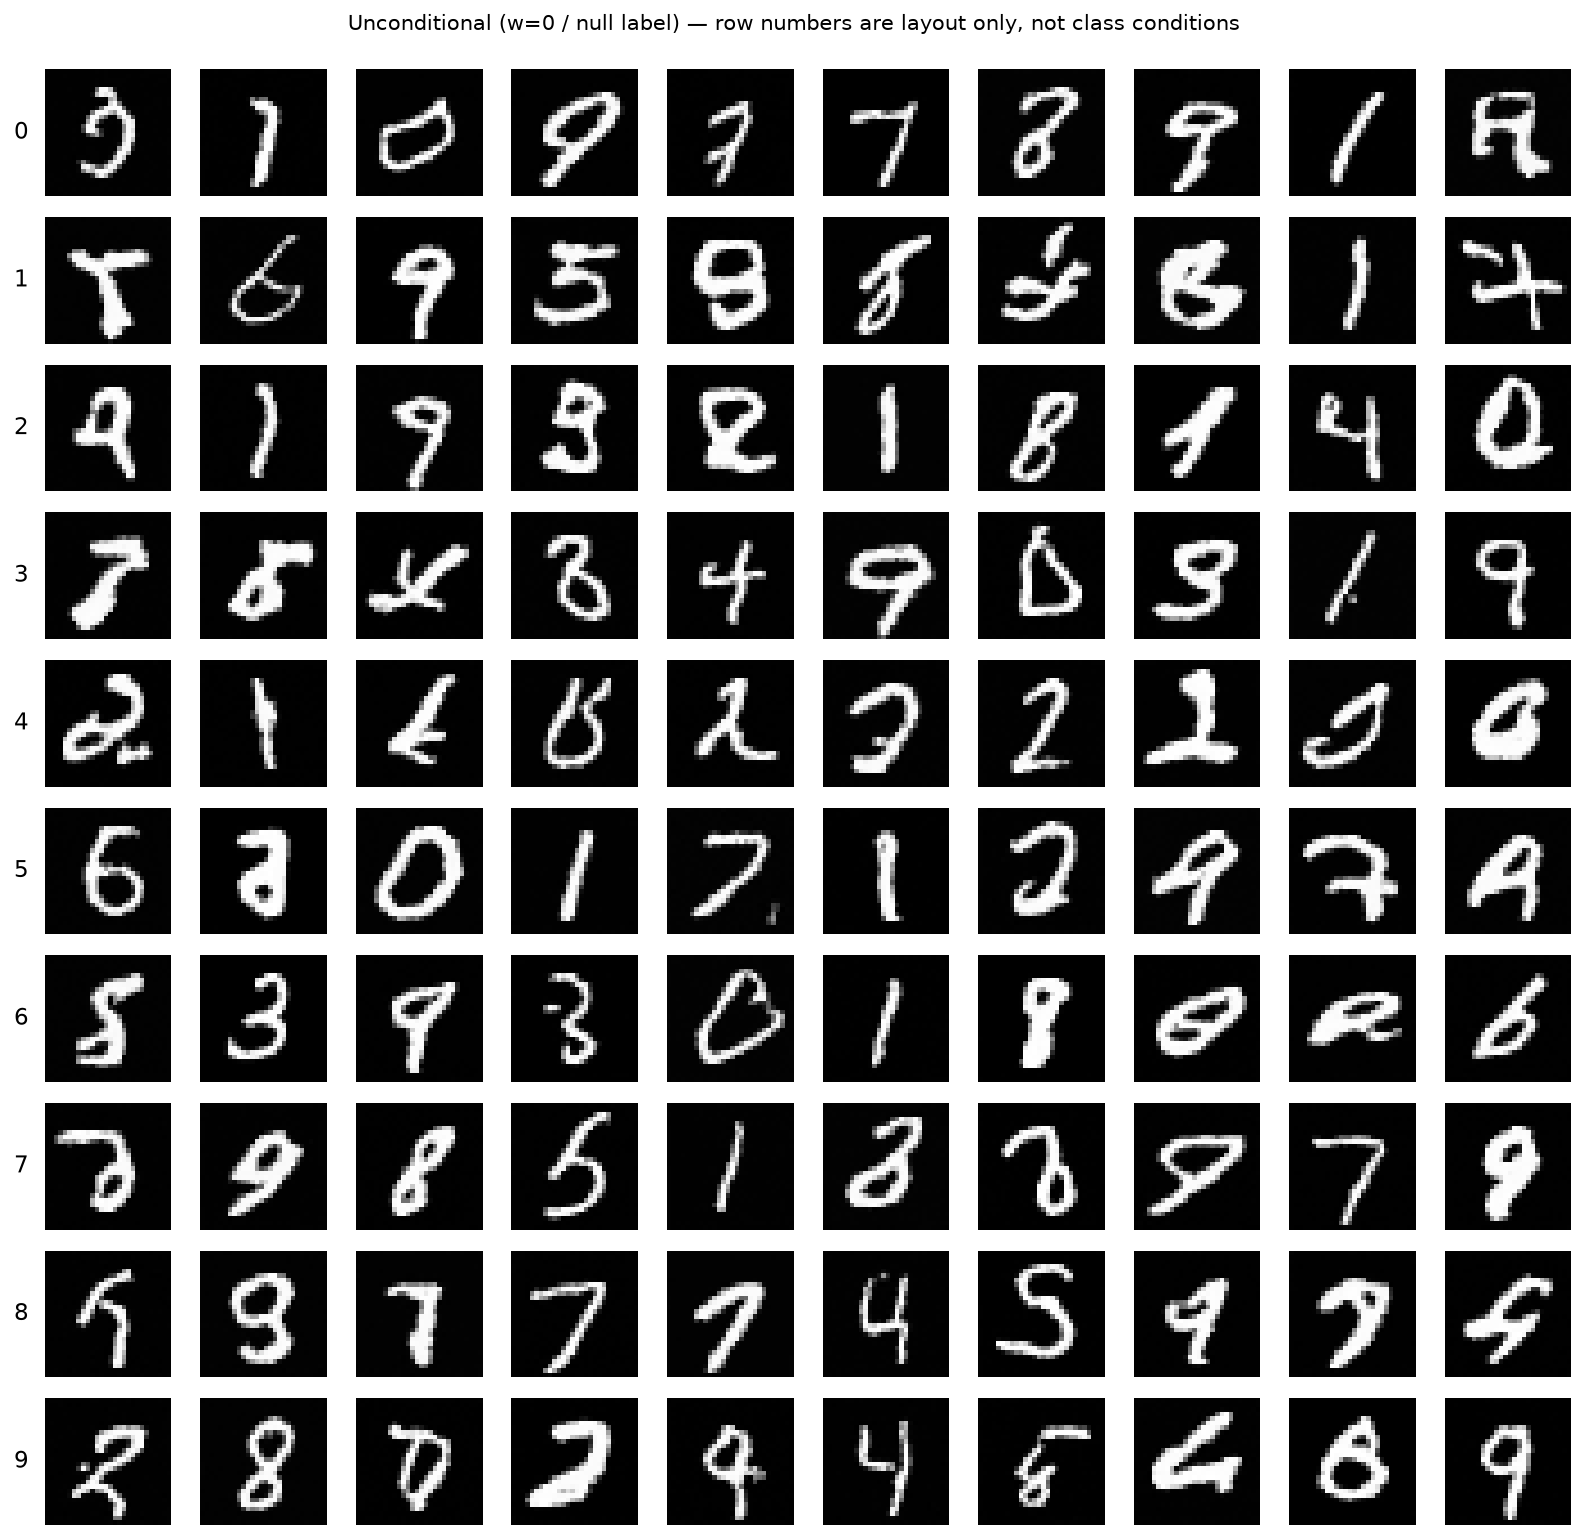
\includegraphics[width=0.72\textwidth]{runs/final/samples_g0.png}
  \caption{无条件采样（null 标签，$w=0$ 等价）。标题已注明：左侧行号仅排版。肉眼可见各行混有 0--9。}
  \label{fig:uncond}
\end{figure}
\begin{figure}[H]
  \centering
  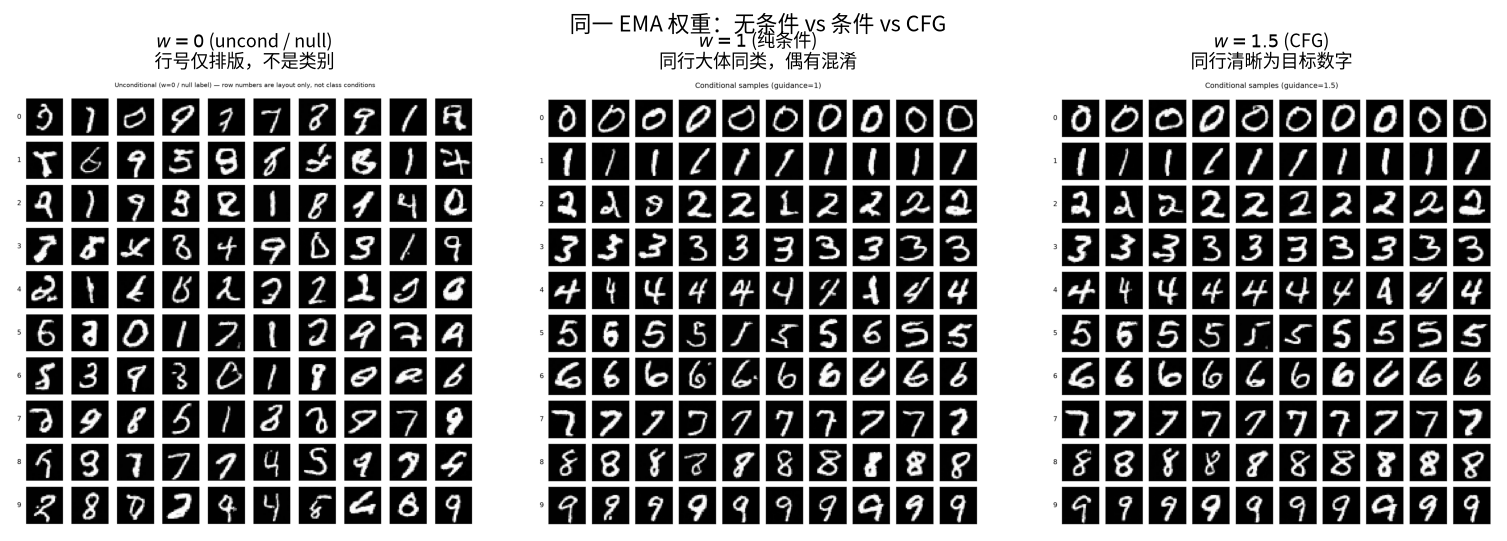
\includegraphics[width=\textwidth]{figs/uncond_vs_cond.png}
  \caption{同一 EMA 权重下 $w=0$ / $1$ / $1.5$ 对照。无条件：数字像 MNIST 但类别随机；条件与 CFG：按行对齐目标数字。}
  \label{fig:uncondcmp}
\end{figure}

\subsubsection{CG 与 CFG 对比}
\begin{center}\small
\renewcommand{\arraystretch}{1.25}
\begin{tabularx}{\linewidth}{@{}p{0.2\linewidth}XX@{}}
\toprule
 & Classifier Guidance（CG） & Classifier-Free Guidance（CFG） \\
\midrule
引导方向 & $\nabla_{\x_t}\log p_\phi(c\mid\x_t)$，外部分类器的输入梯度 & $-(\eps_c-\eps_\emptyset)/\sqrt{1-\abar_t}$，隐式分类器 \\
额外模型 & 需另训噪声感知分类器 $p_\phi(c\mid\x_t,t)$ & 无；同一网络 + null 标签 \\
训练改动 & 扩散模型不变 & 训练时以 $p\approx0.1$ 丢标签 \\
每步采样代价 & 1 次扩散前向 + 分类器前向与反向 & 2 次扩散前向（可拼成一个 batch） \\
风险 & 对抗性梯度、依赖分类器质量 & 大 $w$ 过饱和、多样性下降 \\
可扩展性 & 每种条件要一个分类器 & 任何条件（类别 / 文本 / 图像）通用 \\
代表工作 & ADM（Dhariwal \& Nichol 2021） & GLIDE、Imagen、Stable Diffusion 等 \\
\bottomrule
\end{tabularx}
\end{center}

\subsubsection{代码对照（\code{classroom\_cond\_mnist.py}）}
\begin{lstlisting}[style=py]
# L191-192 training: drop label -> null (10) with p = 0.1
drop = torch.rand(yb.size(0), device=dev) < 0.1
yb = torch.where(drop, torch.full_like(yb, 10), yb)
# L105-110 sampling: cond + uncond in ONE batched forward
if guidance == 1.0:
    e = net(x, t, labels)                                   # plain conditional
else:
    e2 = net(torch.cat([x, x]), torch.cat([t, t]), torch.cat([labels, null]))
    e_c, e_u = e2.float().chunk(2)
    e = e_u + guidance * (e_c - e_u)                        # eq. (CFG)
# L114 then clip x0_hat to [-1, 1] before the posterior mean
\end{lstlisting}
把条件与无条件输入沿 batch 维拼接，一次前向就得到 $\eps_c$ 与 $\eps_\emptyset$，在 GPU 上比两次调用更省时；$w=1$ 时直接跳过无条件分支。

\section{模型架构详解}
本节全部由 \code{train\_cond\_mnist.py} 中的 \code{CondUNet}（\code{base=48, emb\_dim=128}）实例化后逐模块统计得到：输入 $(B,1,28,28)$，参数合计 \textbf{2{,}139{,}713}（与训练日志一致）。采样时使用的是同结构的 EMA 副本（参数逐元素滑动平均，不增加层）。

\begin{sidewaysfigure}
  \centering
  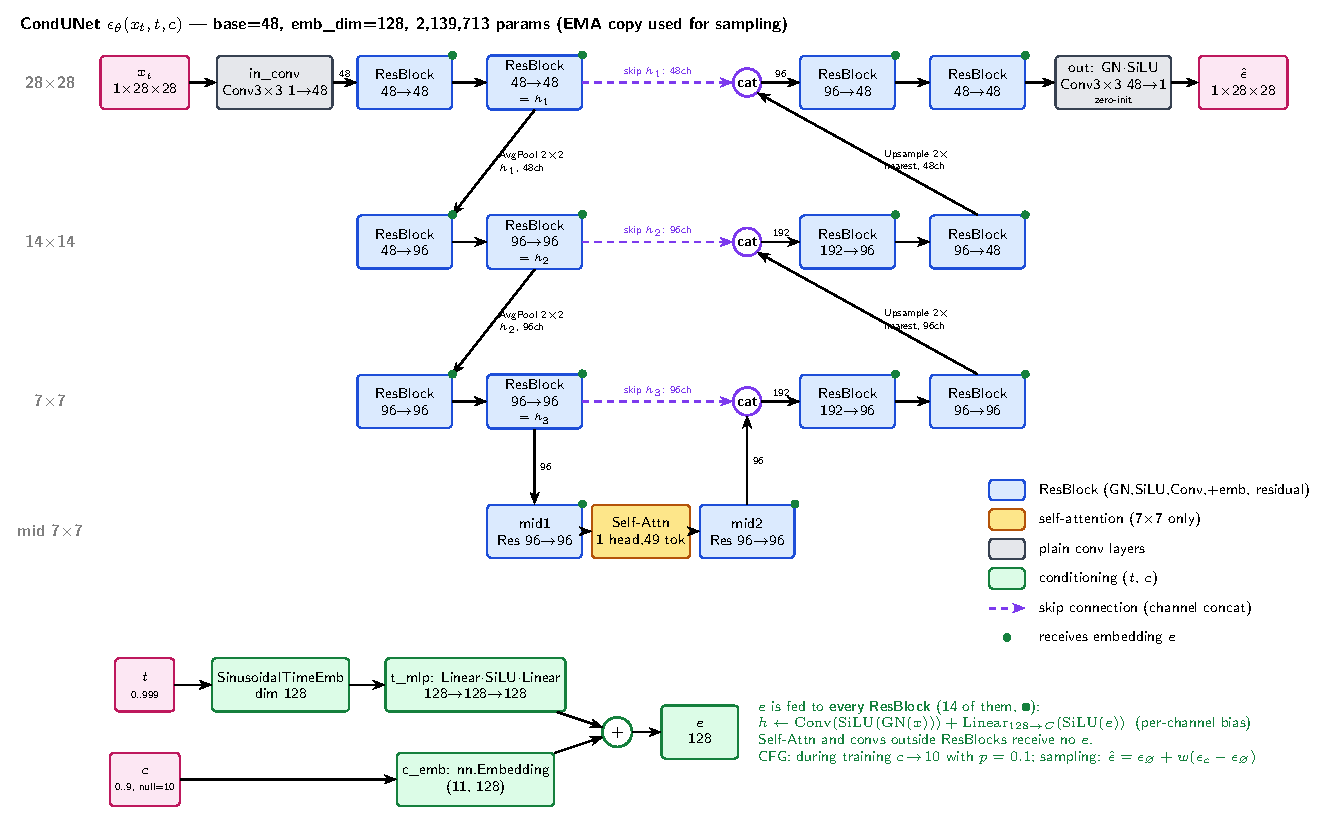
\includegraphics[width=\textheight]{figs/arch/unet_architecture.pdf}
  \caption{\code{CondUNet} 总体架构 $\epst(\x_t,t,c)$。蓝：ResBlock（右上角绿点表示注入了条件向量 $\mathbf e$）；黄：7$\times$7 自注意力；紫色虚线：跳连（通道拼接）；绿：时间 / 类别条件通路。下采样为 AvgPool 2$\times$2（作用在每级第二个块的输出 $h_\ell$ 上），上采样为最近邻 2$\times$。}
  \label{fig:arch}
\end{sidewaysfigure}

\begin{figure}[H]
  \centering
  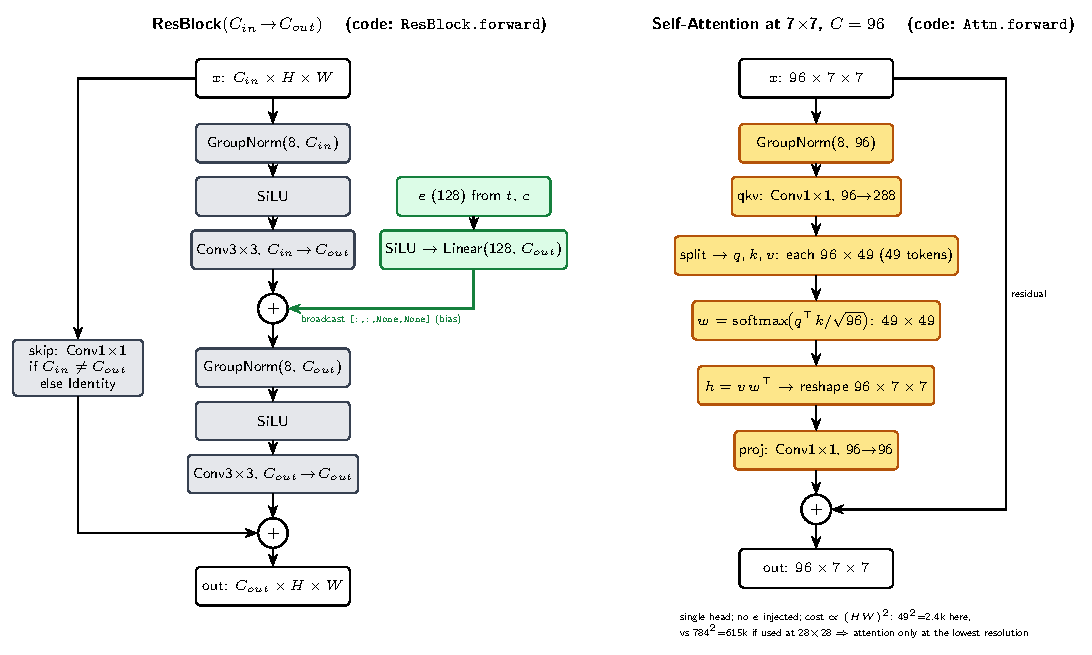
\includegraphics[width=\textwidth]{figs/arch/block_detail.pdf}
  \caption{局部放大。左：ResBlock——条件向量经 SiLU 与 Linear$(128\to C_{out})$ 后作为\emph{逐通道偏置}加在第一个卷积之后（不是 scale-shift）；残差支路在通道数变化时用 1$\times$1 卷积。右：单头自注意力（只在 7$\times$7 使用，不接收 $\mathbf e$）。}
  \label{fig:block}
\end{figure}

\subsection{逐层形状与参数（实测）}
\begin{center}\small
\renewcommand{\arraystretch}{1.12}
\begin{tabular}{@{}llllr@{}}
\toprule
阶段 & 模块（代码名） & 结构 & 输出形状 & 参数 \\
\midrule
条件 & \code{t\_emb} & 正弦时间嵌入 & $128$ & 0 \\
     & \code{t\_mlp} & Linear$\cdot$SiLU$\cdot$Linear & $128$ & 33{,}024 \\
     & \code{c\_emb} & Embedding(11,128) & $128$ & 1{,}408 \\
Stem & \code{in\_conv} & Conv3$\times$3, 1$\to$48 & $48\times28\times28$ & 480 \\
编码 28 & \code{d1.0, d1.1} & ResBlock 48$\to$48 $\times2$ & $48\times28\times28$ & 95{,}904 \\
编码 14 & \code{d2.0, d2.1} & ResBlock 48$\to$96, 96$\to$96 & $96\times14\times14$ & 320{,}832 \\
编码 7 & \code{d3.0, d3.1} & ResBlock 96$\to$96 $\times2$ & $96\times7\times7$ & 357{,}696 \\
瓶颈 & \code{mid1} & ResBlock 96$\to$96 & $96\times7\times7$ & 178{,}848 \\
     & \code{attn} & 单头自注意力 & $96\times7\times7$ & 37{,}440 \\
     & \code{mid2} & ResBlock 96$\to$96 & $96\times7\times7$ & 178{,}848 \\
解码 7 & \code{u3.0, u3.1} & cat(192)$\to$96, 96$\to$96 & $96\times7\times7$ & 459{,}360 \\
解码 14 & \code{u2.0, u2.1} & cat(192)$\to$96, 96$\to$48 & $48\times14\times14$ & 353{,}952 \\
解码 28 & \code{u1.0, u1.1} & cat(96)$\to$48, 48$\to$48 & $48\times28\times28$ & 121{,}392 \\
输出 & \code{out} & GN$\cdot$SiLU$\cdot$Conv3$\times$3 48$\to$1 & $1\times28\times28$ & 529 \\
\midrule
\multicolumn{4}{@{}l}{合计（\code{sum(p.numel())}）} & \textbf{2{,}139{,}713} \\
\bottomrule
\end{tabular}
\end{center}
单个 ResBlock 参数示例：96$\to$96 为 178{,}848（两个 3$\times$3 卷积各 83{,}040，嵌入投影 12{,}384，两个 GroupNorm 各 192）；解码首块 192$\to$96 为 280{,}512（含 1$\times$1 跳连卷积）。参数最多的是 14/7 分辨率的解码端，因为拼接使输入通道翻倍。

\subsection{设计选择：为什么这样搭}
\begin{whybox}
\begin{itemize}[leftmargin=1.2em,itemsep=1pt]
  \item \textbf{多尺度（28$\to$14$\to$7）：}去噪既要全局「这是个几」，又要局部笔画边缘；下采样让感受野迅速覆盖整个数字。
  \item \textbf{跳连拼接：}下采样会丢细节，解码端从编码端 $h_1,h_2,h_3$ 直接拿回同分辨率特征，输出才能有锐利笔画；拼接（而非相加）让后续卷积自己决定如何融合。
  \item \textbf{每个 ResBlock 都注入 $\mathbf e$：}同一个网络要处理从几乎干净（$t\approx0$）到纯噪声（$t\approx T$）的输入，每一层都需要知道「现在噪声多大、要画哪个数字」；只在输入处注入会被深层逐渐稀释。
  \item \textbf{时间 + 类别相加：}两者都映射到 128 维后相加，共用一条条件通道，实现最简单；类别表多一行 null（下标 10），训练时 10\% 概率替换，使同一网络同时学会 $\eps_c$ 与 $\eps_\emptyset$，从而支持 CFG。
  \item \textbf{注意力只放在 7$\times$7：}代价 $\propto(HW)^2$，7$\times$7 只有 49 个 token（$49^2\approx2.4$k），28$\times$28 则为 $784^2\approx61$ 万；在最低分辨率加一层就补上了全局感受野——这正是旧版小网络缺的。
  \item \textbf{GroupNorm：}不依赖 batch 统计，批量小或采样时（\code{eval}）行为与训练一致；8 组适配 48/96 通道。
  \item \textbf{输出卷积零初始化：}训练开始时 $\hat\eps\equiv0$，loss 从 $\approx1$ 平稳下降，不会被随机输出干扰。
  \item \textbf{EMA：}采样用参数的指数滑动平均（衰减 0.999），相当于对最近约 1000 步的权重做平均，样本更平滑稳定；它不改变结构，只多存一份权重。
\end{itemize}
\end{whybox}

\subsection{公式与模块对照}
\begin{center}\small
\renewcommand{\arraystretch}{1.2}
\begin{tabularx}{\linewidth}{@{}p{0.36\linewidth}X@{}}
\toprule
公式中的量 & 网络中的位置 \\
\midrule
$\x_t\in\mathbb R^{1\times28\times28}$ & \code{forward} 的 \code{x}，进入 \code{in\_conv} \\
$t\in\{0,\dots,999\}$ & \code{t\_emb}（正弦）$\to$ \code{t\_mlp} \\
$c\in\{0..9\}$，$\emptyset=10$ & \code{c\_emb = nn.Embedding(11,128)} \\
$\mathbf e(t,c)$ & \code{emb = t\_mlp(t\_emb(t)) + c\_emb(c)} \\
条件如何作用 & 每个 ResBlock：\code{h = conv1(...) + emb(silu(e))[:,:,None,None]} \\
$\epst(\x_t,t,c)$ & \code{out} 的输出，形状同 $\x_t$；训练目标式~\eqref{eq:cond-loss} \\
$\hat\eps$（CFG） & 采样时调用两次网络（$c$ 与 $\emptyset$），按式~\eqref{eq:cfg} 组合 \\
\bottomrule
\end{tabularx}
\end{center}
与双月实验对比：双月实验的 $\epst$ 是输入 $(x,y,t)$ 的小 MLP，没有空间结构、没有类别输入；这里的 U-Net 把同一个 $\epst$ 换成了适合图像的卷积多尺度结构，数学目标完全不变。

\section{教学准备}
\subsection{文件清单（\code{lab\_mnist\_cond.zip}）}
\begin{center}\small
\begin{tabular}{@{}ll@{}}
\toprule
文件 & 用途 \\
\midrule
\code{requirements.txt} & \code{torch, torchvision, numpy, matplotlib} \\
\code{train\_cond\_mnist.py} & 完整训练 + 多 guidance 采样 + 保存 ckpt \\
\code{classroom\_cond\_mnist.py} & 课堂单文件版：\emph{同一个} 2.14M 参数 CondUNet，GPU 加速设置，可投影 \\
\code{runs/final/ckpt\_ema.pt} & 已训练好的 EMA 权重（8.6 MB），免训练直接采样 \\
\code{sample\_by\_digit.py} & 指定单个数字采样，或重出 0–9 网格 \\
\code{eval\_classifier.py} & 小 CNN 分类器给生成样本「判卷」（逐类准确率） \\
\code{runs/final/} & 修复后推荐程（8 epochs）实测产出：网格、$\hat\x_0$ 检查、loss、分类评测 \\
\code{runs/longer/} & 修复\emph{前}旧版（$T=100$，15 epochs）产出，仅作反面对照 \\
\code{figs/} & CFG 对比拼图等 \\
\bottomrule
\end{tabular}
\end{center}

\subsection{环境与运行}
沿用双月实验的 venv 即可，另装 torchvision：
\begin{lstlisting}[style=sh]
# 若尚未安装（需与 torch 同为 CPU 轮）：
pip install torchvision --index-url https://download.pytorch.org/whl/cpu
cd lab_mnist_cond
# 推荐程（默认参数即此设定；本机实测训练 27.5 分钟 + 采样约 7 分钟）
python train_cond_mnist.py --epochs 8 --T 1000 --base 48 --device cpu --out runs/final
# 重出 10x10 网格 / 指定生成数字 3（自动使用 EMA 权重）
python sample_by_digit.py --ckpt runs/final/ckpt.pt --guidance 1.5
python sample_by_digit.py --ckpt runs/final/ckpt.pt --digit 3 --guidance 1.5 --n 16
# 用分类器给生成样本打分（首次会先训一个小 CNN，约 2 分钟）
python eval_classifier.py --ckpt runs/final/ckpt.pt --guidance 1.5 --n 30
\end{lstlisting}
MNIST 首次运行会自动下载到 \code{./data/}（torchvision 开源数据）：\url{https://docs.pytorch.org/vision/stable/generated/torchvision.datasets.MNIST.html}。

\begin{notebox}
\textbf{实测记录（本机 8 核 CPU，PyTorch 2.14.1+cpu，未经挑选）。}
\begin{itemize}[leftmargin=1.4em,itemsep=0pt]
  \item 模型：\code{CondUNet}（每级 2 个 ResBlock，28$\to$14$\to$7，7$\times$7 处单头自注意力），\textbf{2{,}139{,}713} 参数；EMA 衰减 0.999；AdamW，lr $8\times10^{-4}$ + 余弦退火；batch 128。
  \item 日程：线性 $\beta$：$10^{-4}\to0.02$，$T=1000$，$\abar_T\approx4.0\times10^{-5}$。
  \item 训练 8 epochs：\textbf{1649.2 s（27.5 分钟）}，约 205 s/epoch；末 50 步 loss $=\mathbf{0.0220}$（逐轮：0.0293, 0.0259, 0.0243, 0.0230, 0.0226, 0.0221, 0.0215）。
  \item 采样：$\hat\x_0$ 检查 + 3 张 10$\times$10 网格（$w=1,1.5,3$）共 \textbf{424.9 s}。
  \item 结果：100\% 的行都是清晰可读的目标数字（图~\ref{fig:final}）；分类器判卷见表~\ref{tab:clf}。
\end{itemize}
\end{notebox}

\begin{warnbox}
\textbf{本实验第一版的 bug（已修复，留作反面教材）。}第一版用 $T=100$、$\beta:10^{-4}\to0.02$，loss 停在 $\approx0.054$，但生成的「数字」完全认不出（图~\ref{fig:beforeafter} 左）。逐项排查后：
\begin{enumerate}[leftmargin=1.6em,itemsep=0pt]
  \item \textbf{主因：$\abar_T\approx0.36$，采样起点错位。}此时真实 $\x_T=0.6\,\x_0+0.8\,\eps$；MNIST 背景像素 $=-1$，所以训练见过的 $\x_T$ 背景均值约 $-0.6$。采样却从 $\N(\mathbf 0,\I)$ 出发——网络在 $t=T$ 附近从未见过这种输入，整条反向链从一开始就偏离，最后得到糊团、甚至整行全黑。双月实验数据已标准化（均值约 0），所以同样的日程「凑合能用」，换到图像就露馅。修复：$T=1000$，$\abar_T\approx4\times10^{-5}$。
  \item \textbf{次因：网络太小（0.26M、每级 1 个块、无全局感受野）。}只修日程、3 epochs 时样本已成笔画但仍有空白行。升级为 2.1M 参数 U-Net + 7$\times$7 注意力 + EMA 后 8 epochs 即清晰。
  \item \textbf{采样细节：}先算 $\hat\x_0=(\x_t-\sqrt{1-\abar_t}\hat\eps)/\sqrt{\abar_t}$ 并裁剪到 $[-1,1]$，再用后验均值 $\tilde{\boldsymbol\mu}_t(\x_t,\hat\x_0)$ 与后验方差 $\tilde\beta_t$；不裁剪时它与 $\eps$ 形式均值完全相等，裁剪则防止 CFG 外推把像素推出数据范围。
\end{enumerate}
排查中\emph{确认无误}的项：数据缩放 $[-1,1]$ 与保存时 $(x+1)/2$ 一致、$t$ 下标训练/采样都是 0-based、最后一步不加噪、CFG 公式与 null 标签 $=10$、U-Net 跳连形状、保存图像未二次归一化。
\textbf{教训：loss 下降 $\ne$ 采样正确}——loss 只检查「单步去噪」，不检查「采样起点是否与训练分布一致」。必做的健全性检查：$\hat\x_0$ 重建图（图~\ref{fig:x0}）+ 直接看网格。
\end{warnbox}

\section{课堂流程}
\begin{stepbox}{环节 A｜从无条件到有条件（20 分钟）}
\textbf{教师：}回顾双月实验「只能随机生成」。提问：若想「只要数字 7」该怎么办？引出 $p(\x\mid c)$ 与 $\epst(\x_t,t,c)$。板书式 \eqref{eq:cond-loss} 与嵌入公式。\\
\textbf{学生：}对照双月代码，标出「哪里多了 $c$」。\\
\textbf{检查点：}能说出前向不加 $c$、反向 / 网络要加 $c$。
\end{stepbox}

\begin{stepbox}{环节 B｜代码对照（25 分钟）}
\textbf{教师：}投影 \code{classroom\_cond\_mnist.py}，按表~\ref{tab:map} 走读：Embedding、CFG drop、闭式加噪、CFG 采样公式。\\
\textbf{学生：}在第「$e = te(t)+ce(c)$」行旁注释「条件入口」；在 CFG 公式旁写出式 \eqref{eq:cfg}。
\end{stepbox}

\begin{stepbox}{环节 C｜GPU 上现场训练 + 穿插讲解（30 分钟）}
\textbf{教师：}在 A100 / H200 上运行 \code{python classroom\_cond\_mnist.py --epochs 10}（推荐 8–20 epochs）。脚本先打印 \code{params=2,139,713}，每个 epoch 打印 loss、本轮耗时与累计耗时，最后打印 \code{TRAIN DONE} 与采样耗时——\textbf{以屏幕上的真实数字为准}；本教案给出的 GPU 时间（10 epochs 约 2–5 分钟、100 张 $\times$ 1000 步采样约 1 分钟内）只是\emph{估计}。等待期间讲：现场打印 $\abar_T$ 并对比 $T=100$ 时的 $0.36$；U-Net 为何适合图像、GroupNorm、为何归一化到 $[-1,1]$。\\
\textbf{兜底：}时间不够或 GPU 不可用时，运行 \code{python classroom\_cond\_mnist.py --load runs/final/ckpt\_ema.pt}，直接用已训练好的 EMA 权重采样（8 核 CPU 实测：100 张 $\times$ 1000 步、$w=1.5$ 共 256.5 s，网格清晰可读）。\\
\textbf{学生：}观察 loss 是否下降；打开 \code{classroom\_out/samples\_g1.5.png} 与 \code{loss.png}。
\end{stepbox}

\begin{notebox}
\textbf{GPU 使用提示。}
\begin{itemize}[leftmargin=1.4em,itemsep=0pt]
  \item 设备自动选择（\code{--device auto}：有 cuda 用 cuda）；多卡机器用 \code{CUDA\_VISIBLE\_DEVICES=0 python classroom\_cond\_mnist.py ...} 给每位学生 / 每组固定一张卡。
  \item 默认 bf16 autocast（A100/H200 原生支持），\code{--no-amp} 可关闭对照；同时开启 TF32 与 \code{cudnn.benchmark}。
  \item 整个 MNIST（$60000\times28\times28$，约 188 MB float32）一次性放进显存，每步用随机下标切片，不经过 DataLoader，GPU 不会等数据。
  \item 默认 \code{--batch 256}，学习率按 $8\times10^{-4}\sqrt{\text{batch}/128}$ 缩放；可试 512。EMA 衰减 0.999 按步计，batch 越大每 epoch 步数越少，总 epochs 宜相应增加（如 batch 512 用 16–20 epochs）。
  \item \code{--compile} 可选开启 \code{torch.compile}（首次编译需额外时间，默认关闭以求稳妥）。
\end{itemize}
\end{notebox}

\begin{stepbox}{环节 D｜条件采样与 CFG（20 分钟）}
\textbf{教师：}展示图~\ref{fig:final}、\ref{fig:beforeafter}、\ref{fig:cfg}；用 \code{sample\_by\_digit.py --digit 3} 现场要一个「3」。讨论 $w=1,1.5,3$ 的差别。\\
\textbf{学生：}验收清单打勾；讨论第八节问题。
\end{stepbox}

\section{板书公式}
\begin{keybox}
\begin{align}
  &\text{(1) 条件训练：}\quad L=\E\big\|\eps-\epst(\x_t,t,c)\big\|^2, \\
  &\text{(2) 条件入口：}\quad \mathbf e=\mathrm{MLP}(\mathrm{SinTime}(t))+\mathrm{Embed}(c), \\
  &\text{(3) CFG 采样：}\quad \hat\eps=\eps_\emptyset+w(\eps_c-\eps_\emptyset),\quad
    \x_{t-1}=\tfrac{1}{\sqrt{\alpha_t}}\big(\x_t-\tfrac{\beta_t}{\sqrt{1-\abar_t}}\hat\eps\big)+\sigma_t\mathbf z, \\
  &\text{(4) 检查：}\quad \abar_T\approx0\ (T=1000)\ \text{才能从}\ \N(\mathbf 0,\I)\ \text{出发};\quad
    \hat\x_0=\tfrac{\x_t-\sqrt{1-\abar_t}\,\hat\eps}{\sqrt{\abar_t}}.
\end{align}
\end{keybox}

\section{核心代码要点与对照表}
课堂单文件版 \code{classroom\_cond\_mnist.py} 与 \code{train\_cond\_mnist.py} 使用逐行相同的 \code{CondUNet}（可互相加载权重）。下面只列出「条件相关」关键片段（行号对应 \code{classroom\_cond\_mnist.py}）：
\begin{lstlisting}[style=py]
self.c_emb = nn.Embedding(num_classes + 1, emb_dim)   # L65: 0..9 + 10=null (CFG)
emb = self.t_mlp(self.t_emb(t)) + self.c_emb(c)       # L84: time + class
h = h + self.emb(F.silu(emb))[:, :, None, None]       # L40: bias in every ResBlock

drop = torch.rand(yb.size(0), device=dev) < 0.1       # L191-192: drop labels
yb = torch.where(drop, torch.full_like(yb, 10), yb)

e2 = net(torch.cat([x, x]), torch.cat([t, t]), torch.cat([labels, null]))
e_c, e_u = e2.float().chunk(2)                        # L108-110: CFG
e = e_u + guidance * (e_c - e_u)
\end{lstlisting}

\begin{table}[H]
\centering\small
\renewcommand{\arraystretch}{1.25}
\caption{条件相关公式与代码对照（\code{classroom\_cond\_mnist.py} / \code{train\_cond\_mnist.py}）}
\label{tab:map}
\begin{tabularx}{\linewidth}{@{}p{0.32\linewidth}X@{}}
\toprule
公式 / 概念 & 代码位置 \\
\midrule
$\mathrm{Embed}(c)$，$c\in\{0..9,\emptyset\}$ & L65 \code{nn.Embedding(11, 128)}；null 下标 $=10$ \\
$\mathbf e(t,c)$ 注入网络 & L84 \code{emb = t\_mlp(t\_emb(t)) + c\_emb(c)}；L40 ResBlock 内逐通道偏置 \\
日程 $\abar_t$，$T=1000$ & L12--15 \\
闭式 $\x_t=\sqrt{\abar_t}\x_0+\sqrt{1-\abar_t}\eps$ & L195，四维广播 \code{[:,None,None,None]} \\
式 \eqref{eq:cond-loss} & L197 \code{mse\_loss(fwd(xt,t,yb), eps)}（bf16 autocast） \\
训练时 $c\leftarrow\emptyset$ & L191--192 \code{torch.where(drop, 10, yb)}，$p=0.1$ \\
EMA 0.999 & L201 \code{pe.lerp\_(pm, 1-0.999)} \\
式 \eqref{eq:cfg} & L108--110，条件/无条件拼成一个 batch 前向 \\
反向一步 & L114 估计并裁剪 $\hat\x_0$；L115--117 后验均值、方差 $\tilde\beta_t$；最后一步不加噪 \\
\bottomrule
\end{tabularx}
\end{table}

\section{预期结果（实测图）}
\begin{figure}[H]
  \centering
  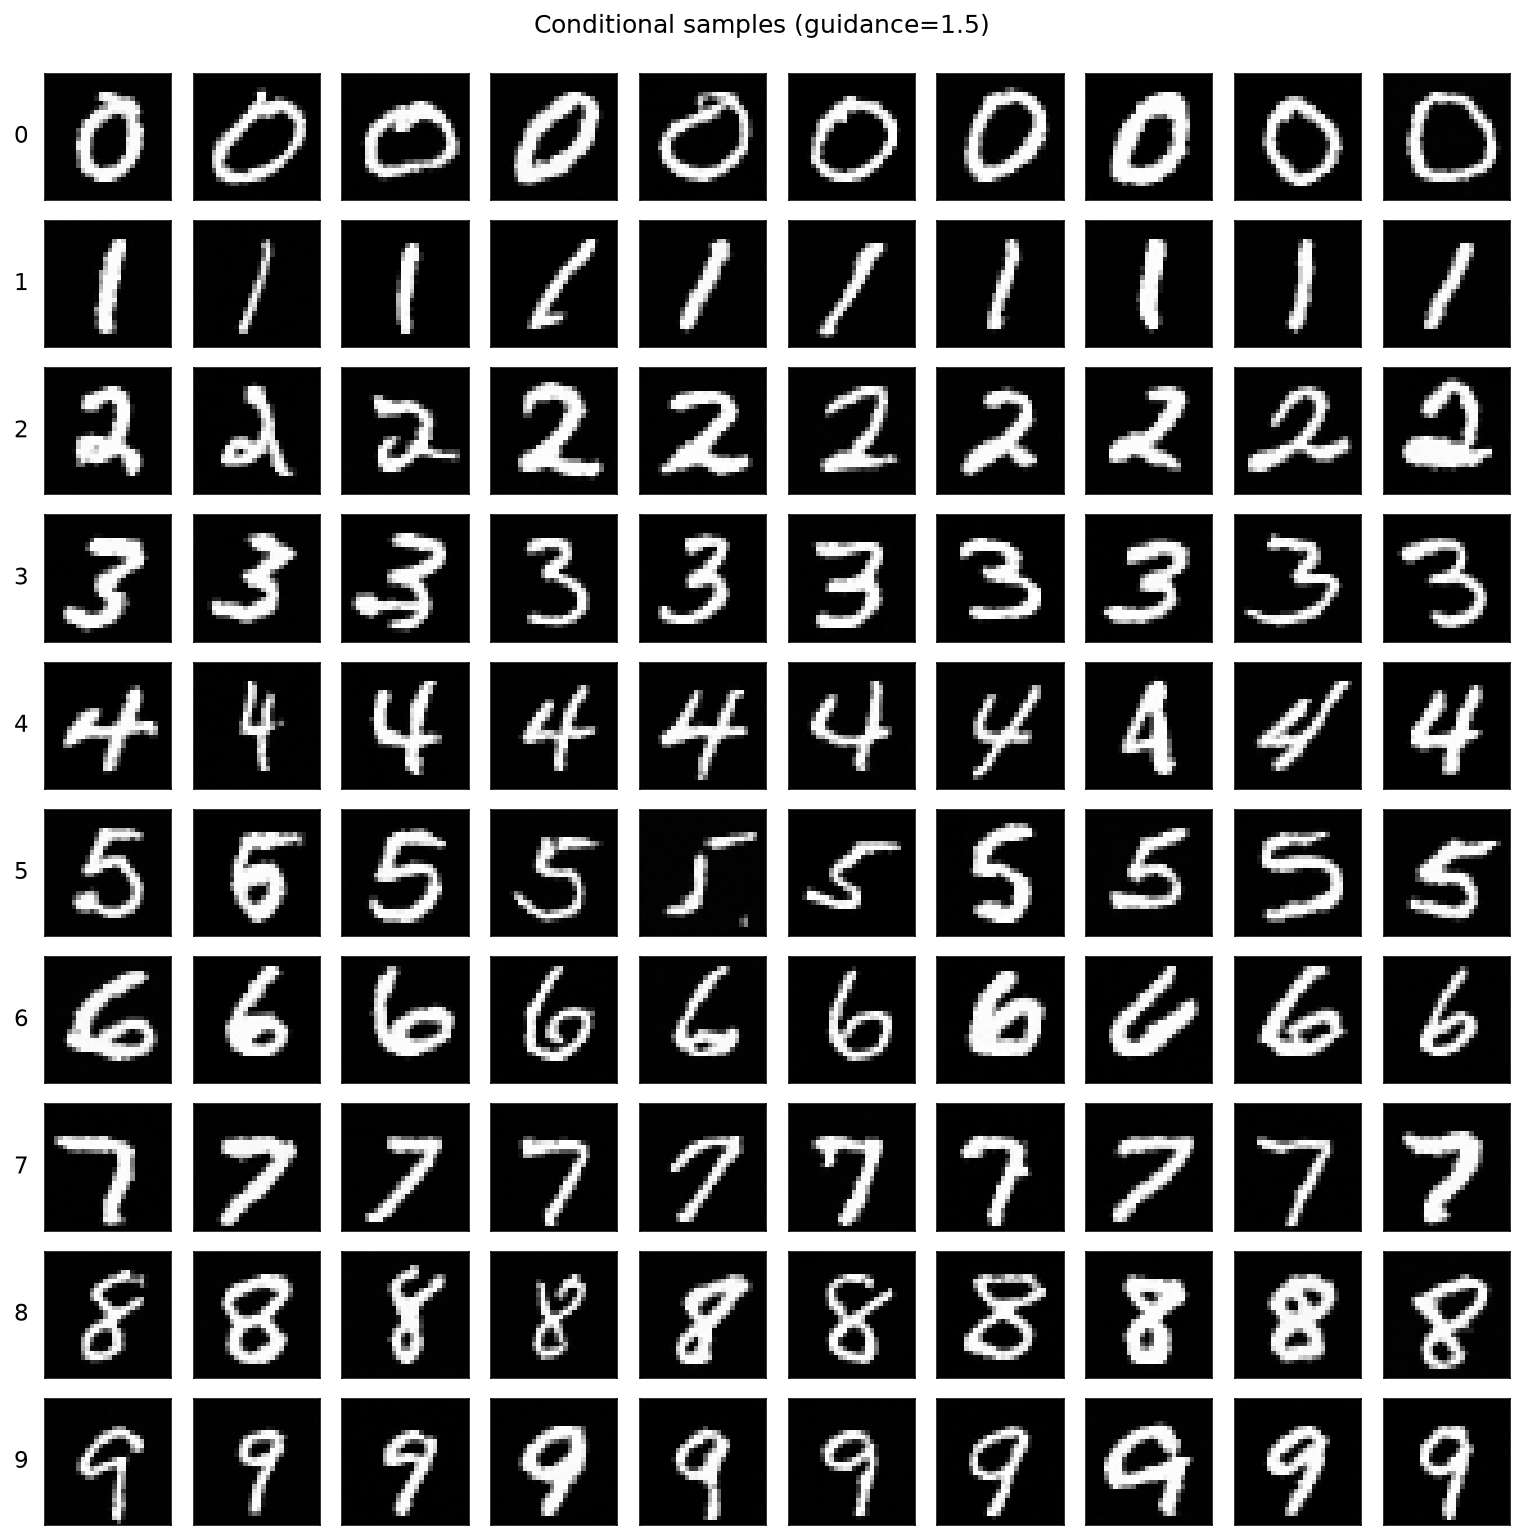
\includegraphics[width=0.72\textwidth]{runs/final/samples_g1.5.png}
  \caption{修复后推荐程（8 epochs，27.5 分钟，EMA 权重，$w=1.5$）10$\times$10 条件网格，各行为条件数字 0–9。未挑选。}
  \label{fig:final}
\end{figure}

\begin{figure}[H]
  \centering
  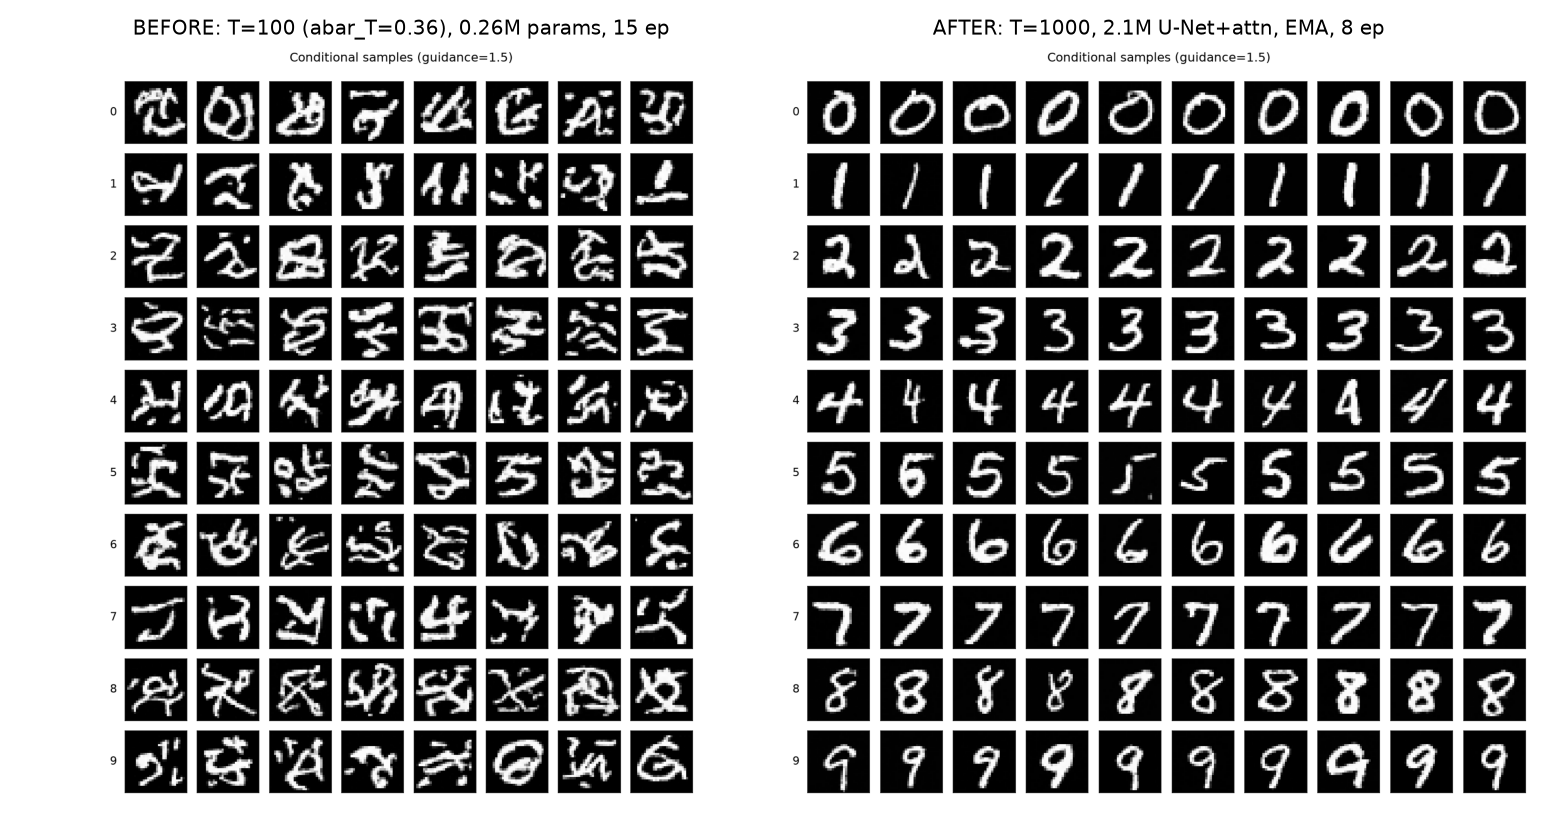
\includegraphics[width=\textwidth]{figs/before_after.png}
  \caption{修复前（左：$T=100$、0.26M 参数、15 epochs）与修复后（右）的同一可视化。左侧 loss 已平台化却认不出数字。}
  \label{fig:beforeafter}
\end{figure}

\begin{figure}[H]
  \centering
  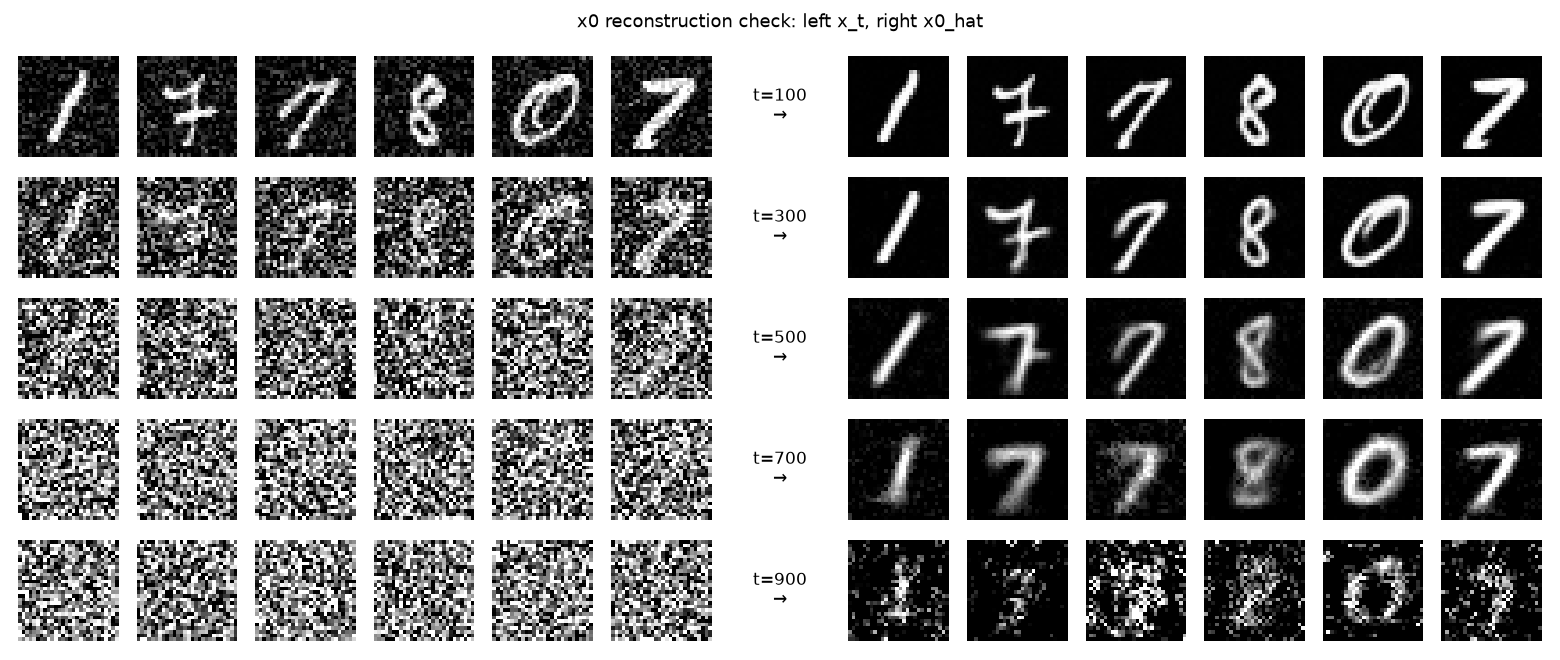
\includegraphics[width=\textwidth]{runs/final/x0_recon_check.png}
  \caption{$\hat\x_0$ 重建检查：真实图加噪到 $t$（左），用预测噪声一步闭式估计 $\hat\x_0$（右）。$t\le700$ 仍能认出原数字，说明网络与日程正确；$t=900$ 时信息几乎被噪声抹掉，需多步采样。}
  \label{fig:x0}
\end{figure}

\begin{figure}[H]
  \centering
  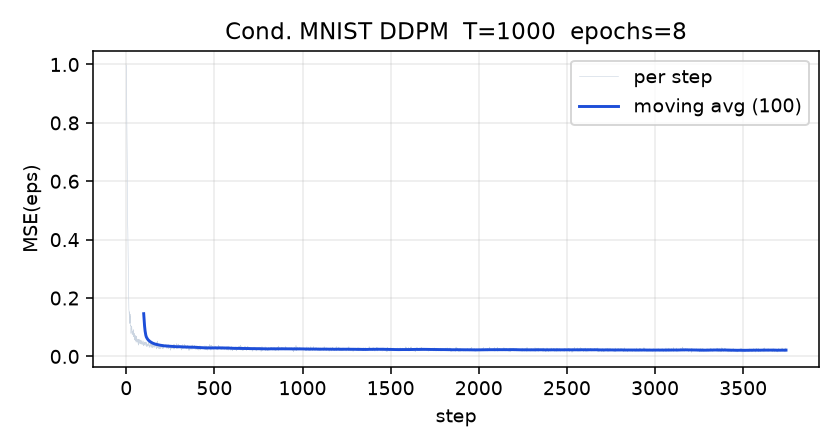
\includegraphics[width=0.55\textwidth]{runs/final/loss.png}
  \caption{训练 loss（灰：逐步；蓝：100 步滑动平均），8 epochs 共 3744 步，末段约 $0.022$。注意 $T$ 不同的 loss 不可直接比较。}
  \label{fig:loss}
\end{figure}

\begin{figure}[H]
  \centering
  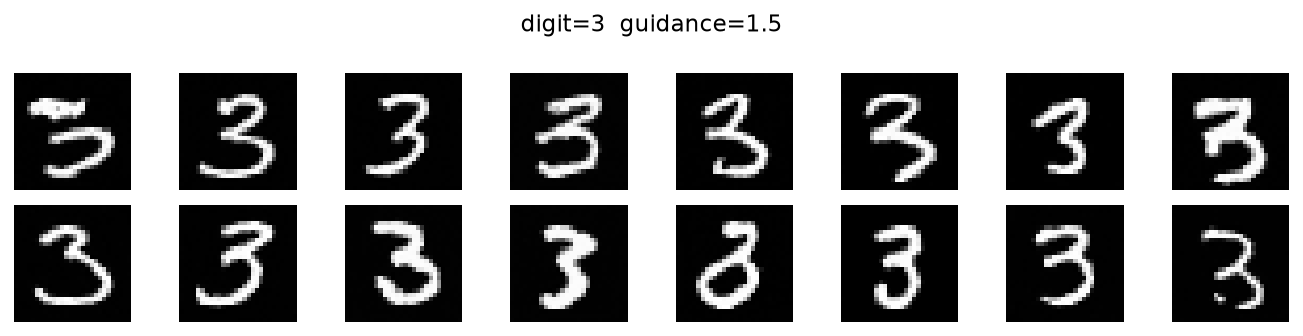
\includegraphics[width=0.55\textwidth]{runs/final/digit_3_g1.5.png}
  \caption{\code{sample\_by\_digit.py --digit 3 --guidance 1.5 --n 16}（修复后模型）。}
  \label{fig:digit3}
\end{figure}

\begin{figure}[H]
  \centering
  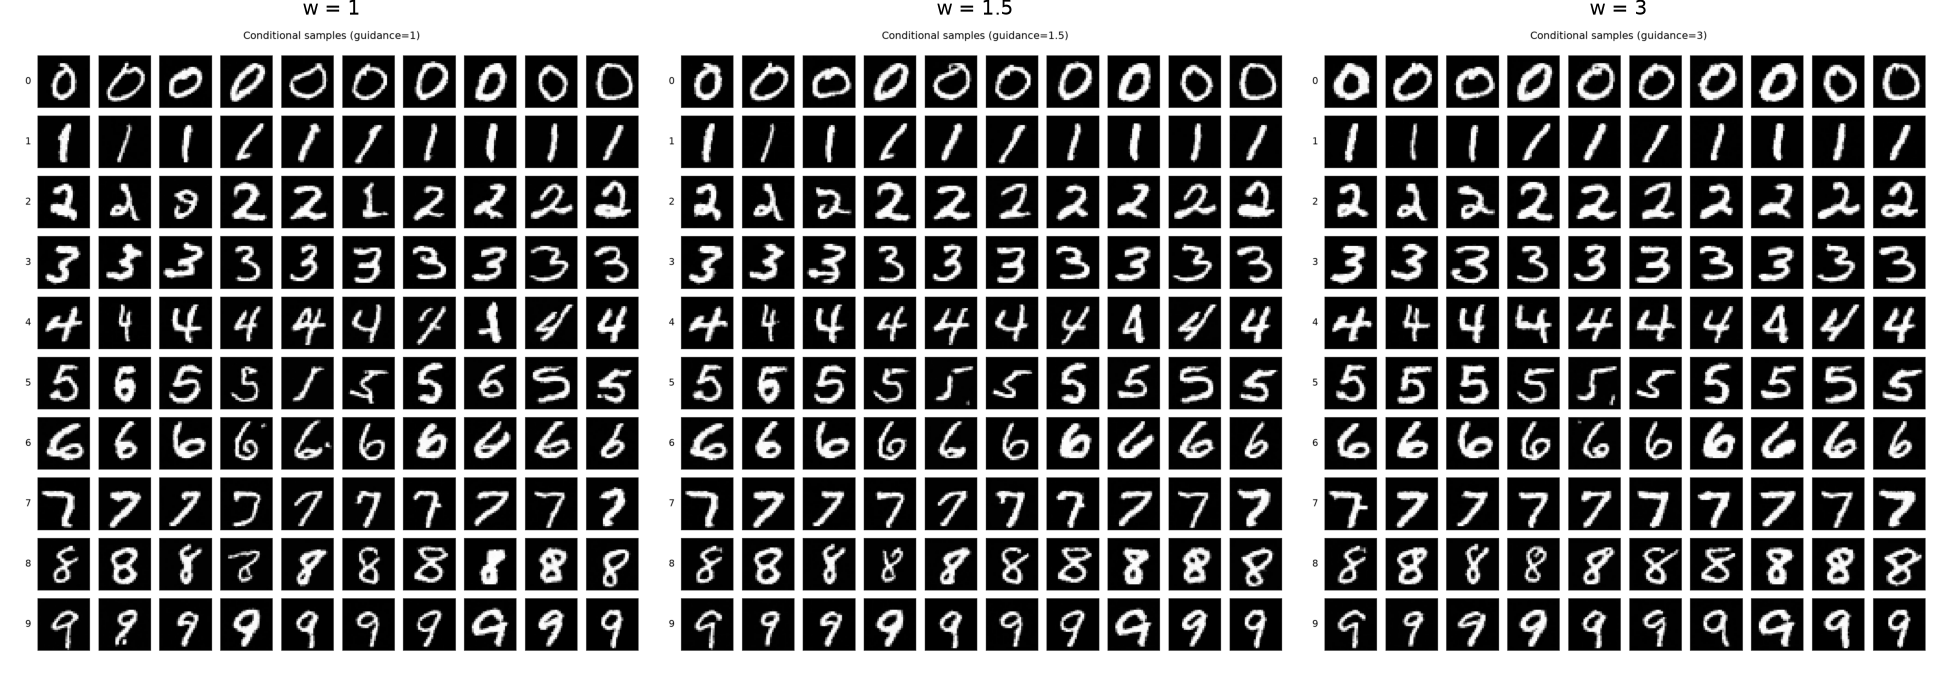
\includegraphics[width=\textwidth]{figs/cfg_compare_final.png}
  \caption{同一模型、同一随机种子下 $w=1,\ 1.5,\ 3$。$w=1$ 偶有类别混淆（如第 2 行出现 1/8 状、第 5 行出现 6 状），$w$ 增大后更「典型」、笔画更粗、多样性下降。}
  \label{fig:cfg}
\end{figure}

\begin{table}[H]
\centering\small
\caption{分类器判卷：小 CNN（MNIST 测试集准确率 98.83\%，训练 2 epochs / 45 s）对生成样本逐类判别（每类 30 张，EMA 权重，未挑选）。}
\label{tab:clf}
\setlength{\tabcolsep}{3.2pt}
\begin{tabular}{@{}l*{10}{c}c@{}}
\toprule
$w$ & 0 & 1 & 2 & 3 & 4 & 5 & 6 & 7 & 8 & 9 & 总体 \\
\midrule
1   & 30/30 & 30/30 & 28/30 & 28/30 & 28/30 & 26/30 & 30/30 & 29/30 & 28/30 & 28/30 & \textbf{95.0\%} \\
1.5 & 30/30 & 30/30 & 30/30 & 30/30 & 30/30 & 30/30 & 30/30 & 30/30 & 30/30 & 30/30 & \textbf{100\%} \\
\bottomrule
\end{tabular}
\end{table}
$w=1$ 时最弱的是数字 5（26/30，常被画成 6 状），与图~\ref{fig:cfg} 的肉眼观察一致；$w=1.5$ 的 300 张全部判对。采样耗时：$w=1.5$ 300 张 1201 s，$w=1$ 300 张 707 s（$w=1$ 无需无条件前向）。

\section{验收清单}
\begin{itemize}[leftmargin=1.6em,itemsep=1pt]
  \item[$\square$] 打印的 $\abar_T$ 接近 0（本实验 $4\times10^{-5}$）；loss 降到约 $0.02$ 量级；
  \item[$\square$] $\hat\x_0$ 检查图中 $t\le500$ 能认出原数字；
  \item[$\square$] 0–9 网格\textbf{每行至少 8/10 张肉眼可读且为目标数字}；
  \item[$\square$] 看过 $w=0$ 无条件网格（图~\ref{fig:uncond}）：仍是数字，但类别混杂——理解「条件」的作用；
  \item[$\square$] \code{sample\_by\_digit.py --digit 3} 得到的图均为「3」（图~\ref{fig:digit3}）；
  \item[$\square$] 能指出条件入口那一行，并能解释 CFG 公式中 $w$ 的作用；
  \item[$\square$] 能说明：本实验与双月实验共享哪些公式、多了什么。
\end{itemize}

\section{讨论与作业}
\begin{enumerate}[leftmargin=2em,itemsep=2pt]
  \item 无条件模型能否「只要 7」？需要什么额外机制？
  \item 若训练时\emph{从不}丢掉标签（$p_{\mathrm{uncond}}=0$），CFG 还能用吗？为什么？
  \item 把 guidance 设为 $0$，对应公式里什么？生成的还是指定数字吗？
  \item \textbf{作业：}用 \code{--T 100} 重训（其余不变），复现图~\ref{fig:beforeafter} 左侧的失败，并打印 $\x_T$ 背景均值解释原因；或把条件从「类别」换成「奇偶」二分类，观察是否仍可控。
\end{enumerate}

\section{常见问题}
\begin{center}\small
\renewcommand{\arraystretch}{1.3}
\begin{tabularx}{\linewidth}{@{}>{\raggedright\arraybackslash}p{0.32\linewidth}X@{}}
\toprule
现象 & 原因与处理 \\
\midrule
所有行长得差不多 & 条件没喂进网络（忘了 \code{+ ce(c)}），或采样时 labels 全是同一值。 \\
loss 平台化但数字认不出 & 先查 $\abar_T$：$T=100$ 时 $\abar_T\approx0.36$，采样起点与训练错位（本实验第一版的 bug）；再看 $\hat\x_0$ 检查图。 \\
某几行整行全黑 / 空白 & 同上；或网络太小 + CFG 外推过度且未裁剪 $\hat\x_0$。 \\
指定 3 却像噪声 & 训练太短、采样用了未训练的权重（忘加载 EMA / ckpt），或 guidance 为 0。 \\
\code{Embedding} 报错 index 10 & \code{Embedding} 大小须为 11（0..9+null）。 \\
图像全白 / 全黑 & 忘了 Normalize 到 $[-1,1]$，或保存前没做 \code{(x+1)/2}。 \\
torchvision 与 torch 不匹配 & 用同一 CPU 轮安装：\code{pip install torchvision --index-url https://download.pytorch.org/whl/cpu}。 \\
没时间训练 & \code{classroom\_cond\_mnist.py --load runs/final/ckpt\_ema.pt}，直接用已训练好的 EMA 权重采样。 \\
\bottomrule
\end{tabularx}
\end{center}

\section{与双月教案、数学讲义的衔接}
\begin{center}\small
\renewcommand{\arraystretch}{1.25}
\begin{tabularx}{\linewidth}{@{}>{\raggedright\arraybackslash}p{0.36\linewidth}X@{}}
\toprule
本实验 & 对应材料 \\
\midrule
前向闭式、$\eps$-loss、祖先采样 & 双月教案第四–五节；讲义式 (2.4)、(4.9)、算法 1–2 \\
重参数化构造 $\x_t$ & 讲义 §2.4；双月代码第 50 行同构 \\
条件分布 $p(\x\mid c)$ & 讲义「反向匹配后验」在条件数据上的自然推广 \\
CFG & Ho \& Salimans 2022；与讲义 score 观点：引导 = 沿条件得分方向加大步长 \\
\bottomrule
\end{tabularx}
\end{center}
\textbf{建议顺序：}双月无条件跑通 $\to$ 本条件 MNIST $\to$ 回到讲义第三章理解「反向一步为何像高斯」$\to$ 课外 Diffusers 文生图教程。

\section{参考资料与链接}
\small
\begin{enumerate}[label={[\arabic*]},leftmargin=2.2em,itemsep=2pt]
  \item J. Ho et al. Denoising Diffusion Probabilistic Models. \url{https://arxiv.org/abs/2006.11239}
  \item J. Ho, T. Salimans. Classifier-Free Diffusion Guidance. \url{https://arxiv.org/abs/2207.12598}
  \item P. Dhariwal, A. Nichol. Diffusion Models Beat GANs on Image Synthesis（Classifier Guidance）. \url{https://arxiv.org/abs/2105.05233}
  \item torchvision MNIST：\url{https://docs.pytorch.org/vision/stable/generated/torchvision.datasets.MNIST.html}
  \item Hugging Face Diffusers — Conditional image generation：\url{https://huggingface.co/docs/diffusers/using-diffusers/conditional_image_generation}
  \item Diffusers — Classifier-Free Guidance 说明：\url{https://huggingface.co/docs/diffusers/using-diffusers/classifier_free_guidance}
  \item Diffusers 基础训练教程：\url{https://huggingface.co/docs/diffusers/tutorials/basic_training}
  \item PyTorch 安装：\url{https://pytorch.org/get-started/locally/}
  \item 前置教案：同目录上一份 \code{lab\_2d\_ddpm/diffusion\_lab\_lesson\_plan.pdf}
  \item 配套数学讲义：\code{diffusion\_math\_teaching\_notes\_latex.pdf}
\end{enumerate}
{\footnotesize\color{cmuted} 外链均于 2026-10-10 访问验证（HTTP 200）。}

\end{document}
